\documentclass[border=10pt]{standalone}

\usepackage{tikz}
\usepackage{tikzsymbols}
\usetikzlibrary{calc,patterns,shapes.geometric}

\def\centerarc[#1](#2)(#3:#4:#5){\draw[#1] ($(#2)+({#5*cos(#3)},{#5*sin(#3)})$) arc (#3:#4:#5);}

\begin{document}
	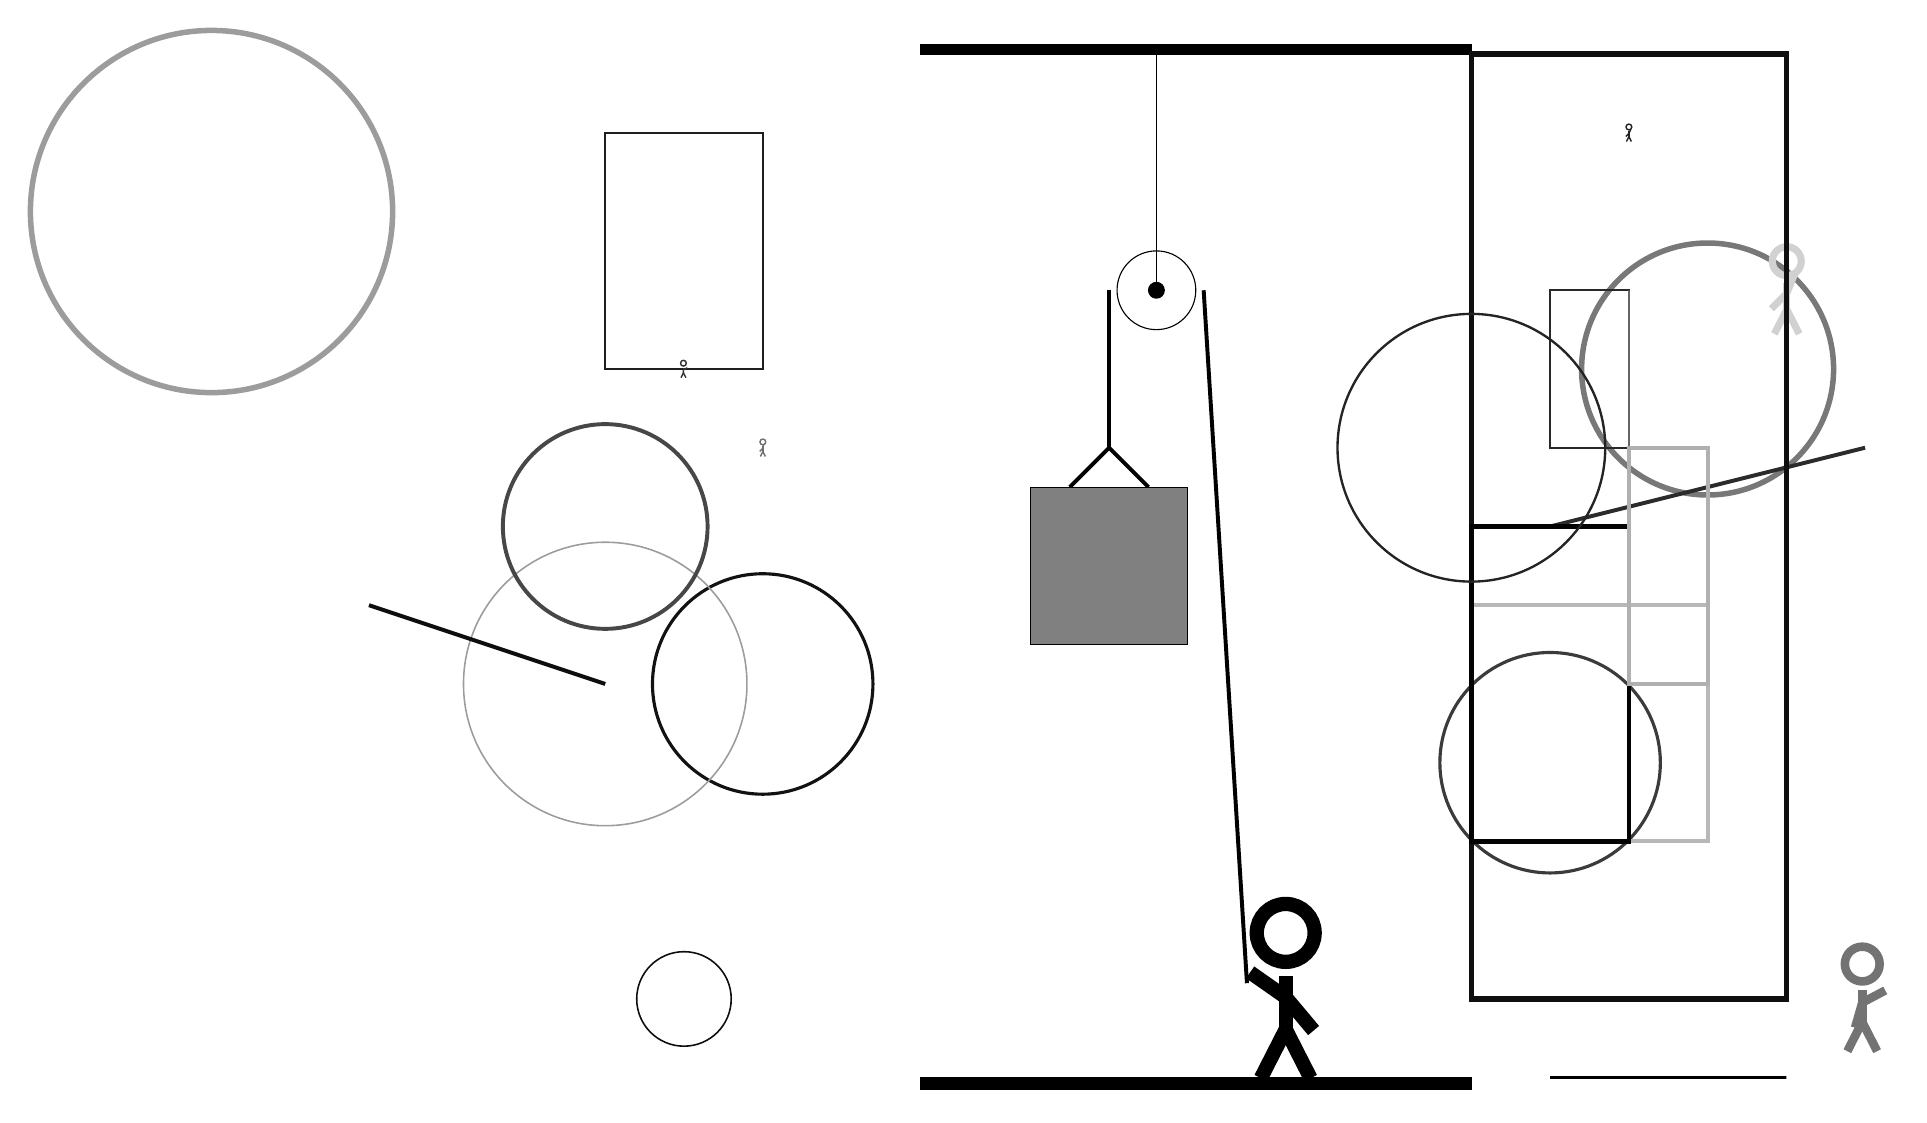
\begin{tikzpicture}
		%%%%% START %%%%%
		
		\draw[fill=black] (-2, 10) rectangle (5, 10.125);
		
		\draw (1, 7) circle (0.5);
		\draw[fill=black] (1, 7) circle (0.1);
		\draw (1, 10) -- (1, 7);
		
		\draw[line width=0.5mm] (-0.1, 4.5) -- (0.4, 5.0) -- (0.9, 4.5);
		\draw[fill=black!50] (-0.6, 4.5) rectangle (1.4, 2.5);
		
		\draw[line width=0.3mm, color=black!88] (-4, 6) rectangle (-6, 9);
		
		\node[line width=0.2mm, color=black!56] at (-4, 5) {\Strichmaxerl[1][43][78]};
		\draw [line width=0.7mm, color=black!53](8, 6) circle (1.6);
		\draw [line width=0.4mm, color=black!77](6, 1) circle (1.4);
		\node[line width=0.6mm, color=black!18] at (9, 7) {\Strichmaxerl[5][45][68]};
		
		\draw [line width=0.4mm, color=black!93](-4, 2) circle (1.4);
		\draw[line width=0.5mm, color=black!83](6, 4) -- (10, 5);
		\draw [line width=0.2mm, color=black!39](-6, 2) circle (1.8);
		\draw[line width=0.5mm, color=black!28] (5, 0) rectangle (8, 3);
		\node[line width=0.3mm, color=black!86] at (7, 9) {\Strichmaxerl[1][46][65]};
		\draw[line width=0.2mm, color=black!84] (7, 5) rectangle (6, 7);
		
		\draw [line width=0.2mm, color=black!95](-5, -2) circle (0.6);
		\draw[line width=0.5mm, color=black!95](-6, 2) -- (-9, 3);
		\draw[line width=0.2mm, color=black!60] (7, 7) rectangle (7, 4);
		\node[line width=0.3mm, color=black!55] at (10, -2) {\Strichmaxerl[6][74][28]};
		\draw [line width=0.5mm, color=black!72](-6, 4) circle (1.3);
		
		\draw [line width=0.7mm, color=black!39](-11, 8) circle (2.3);
		
		\draw[line width=0.7mm, color=black!94] (5, 10) rectangle (9, -2);
		\draw[line width=0.3mm, color=black!100] (6, -3) rectangle (9, -3);
		\draw[line width=0.6mm, color=black!99] (7, 0) rectangle (5, 4);
		\draw [line width=0.7mm, color=black!98](-4, 7) circle (0.0);
		
		\node[line width=0.4mm, color=black!80] at (-5, 6) {\Strichmaxerl[1][87][25]};
		\draw[line width=0.5mm, color=black!31] (7, 2) rectangle (8, 5);
		\draw [line width=0.3mm, color=black!86](5, 5) circle (1.7);
		
		\draw[line width=0.5mm] (0.4, 7) -- (0.4, 5.0);
		\centerarc[line width=0.5mm](1, 7)(0:180:0.6);
		\draw[line width=0.5mm](1.6, 7) -- (2.15, -1.8);
		
		\node at (2.6, -1.9) {\Strichmaxerl[10][-35][-50]};
		
		\draw[fill=black] (-2, -3) rectangle (5, -3.15);
		
		%%%%% END %%%%%
	\end{tikzpicture}
\end{document}